\section{Simulation Results and Discussion}
\subsection{Stop-and-go waves on a free road}
Our implementation successfully reproduces an unstable traffic and apparition of a jam on an unobstructed road. See figure \ref{fig:free_road} for a representation of the flow. The vehicles start from stand-still, and reach equilibrium velocity within less than a minute. At about $t=\SI{700}{s}$ two seemingly independent perturbations start to grow in intensity, and develop into full blown stop-and-go waves at $t\approx \SI{1100}☺{s}$.

In the IDM, drivers only look at the vehicle \emph{ahead} of them, i.e. information only spreads upstream. Indeed, we observe that the waves travel in direction opposite to the traffic, which means that the information is spread significantly faster than the speed at which the cars are travelling downstream.

We have verified that the waves visible in fig. \ref{fig:free_road} are \emph{not} a numerical artefact, as the same pattern can be observed for very different time steps. In particular, we could reproduce this plot with a time step as small as \SI{1e-4}{s}.

The pattern shown in the simulation is qualitatively very similar to what has recently been experimentally observed by Nakayama et al. \cite{nakayama2009} and Tadaki et al. \cite{tadaki2013}.
\begin{figure}
    \centering
    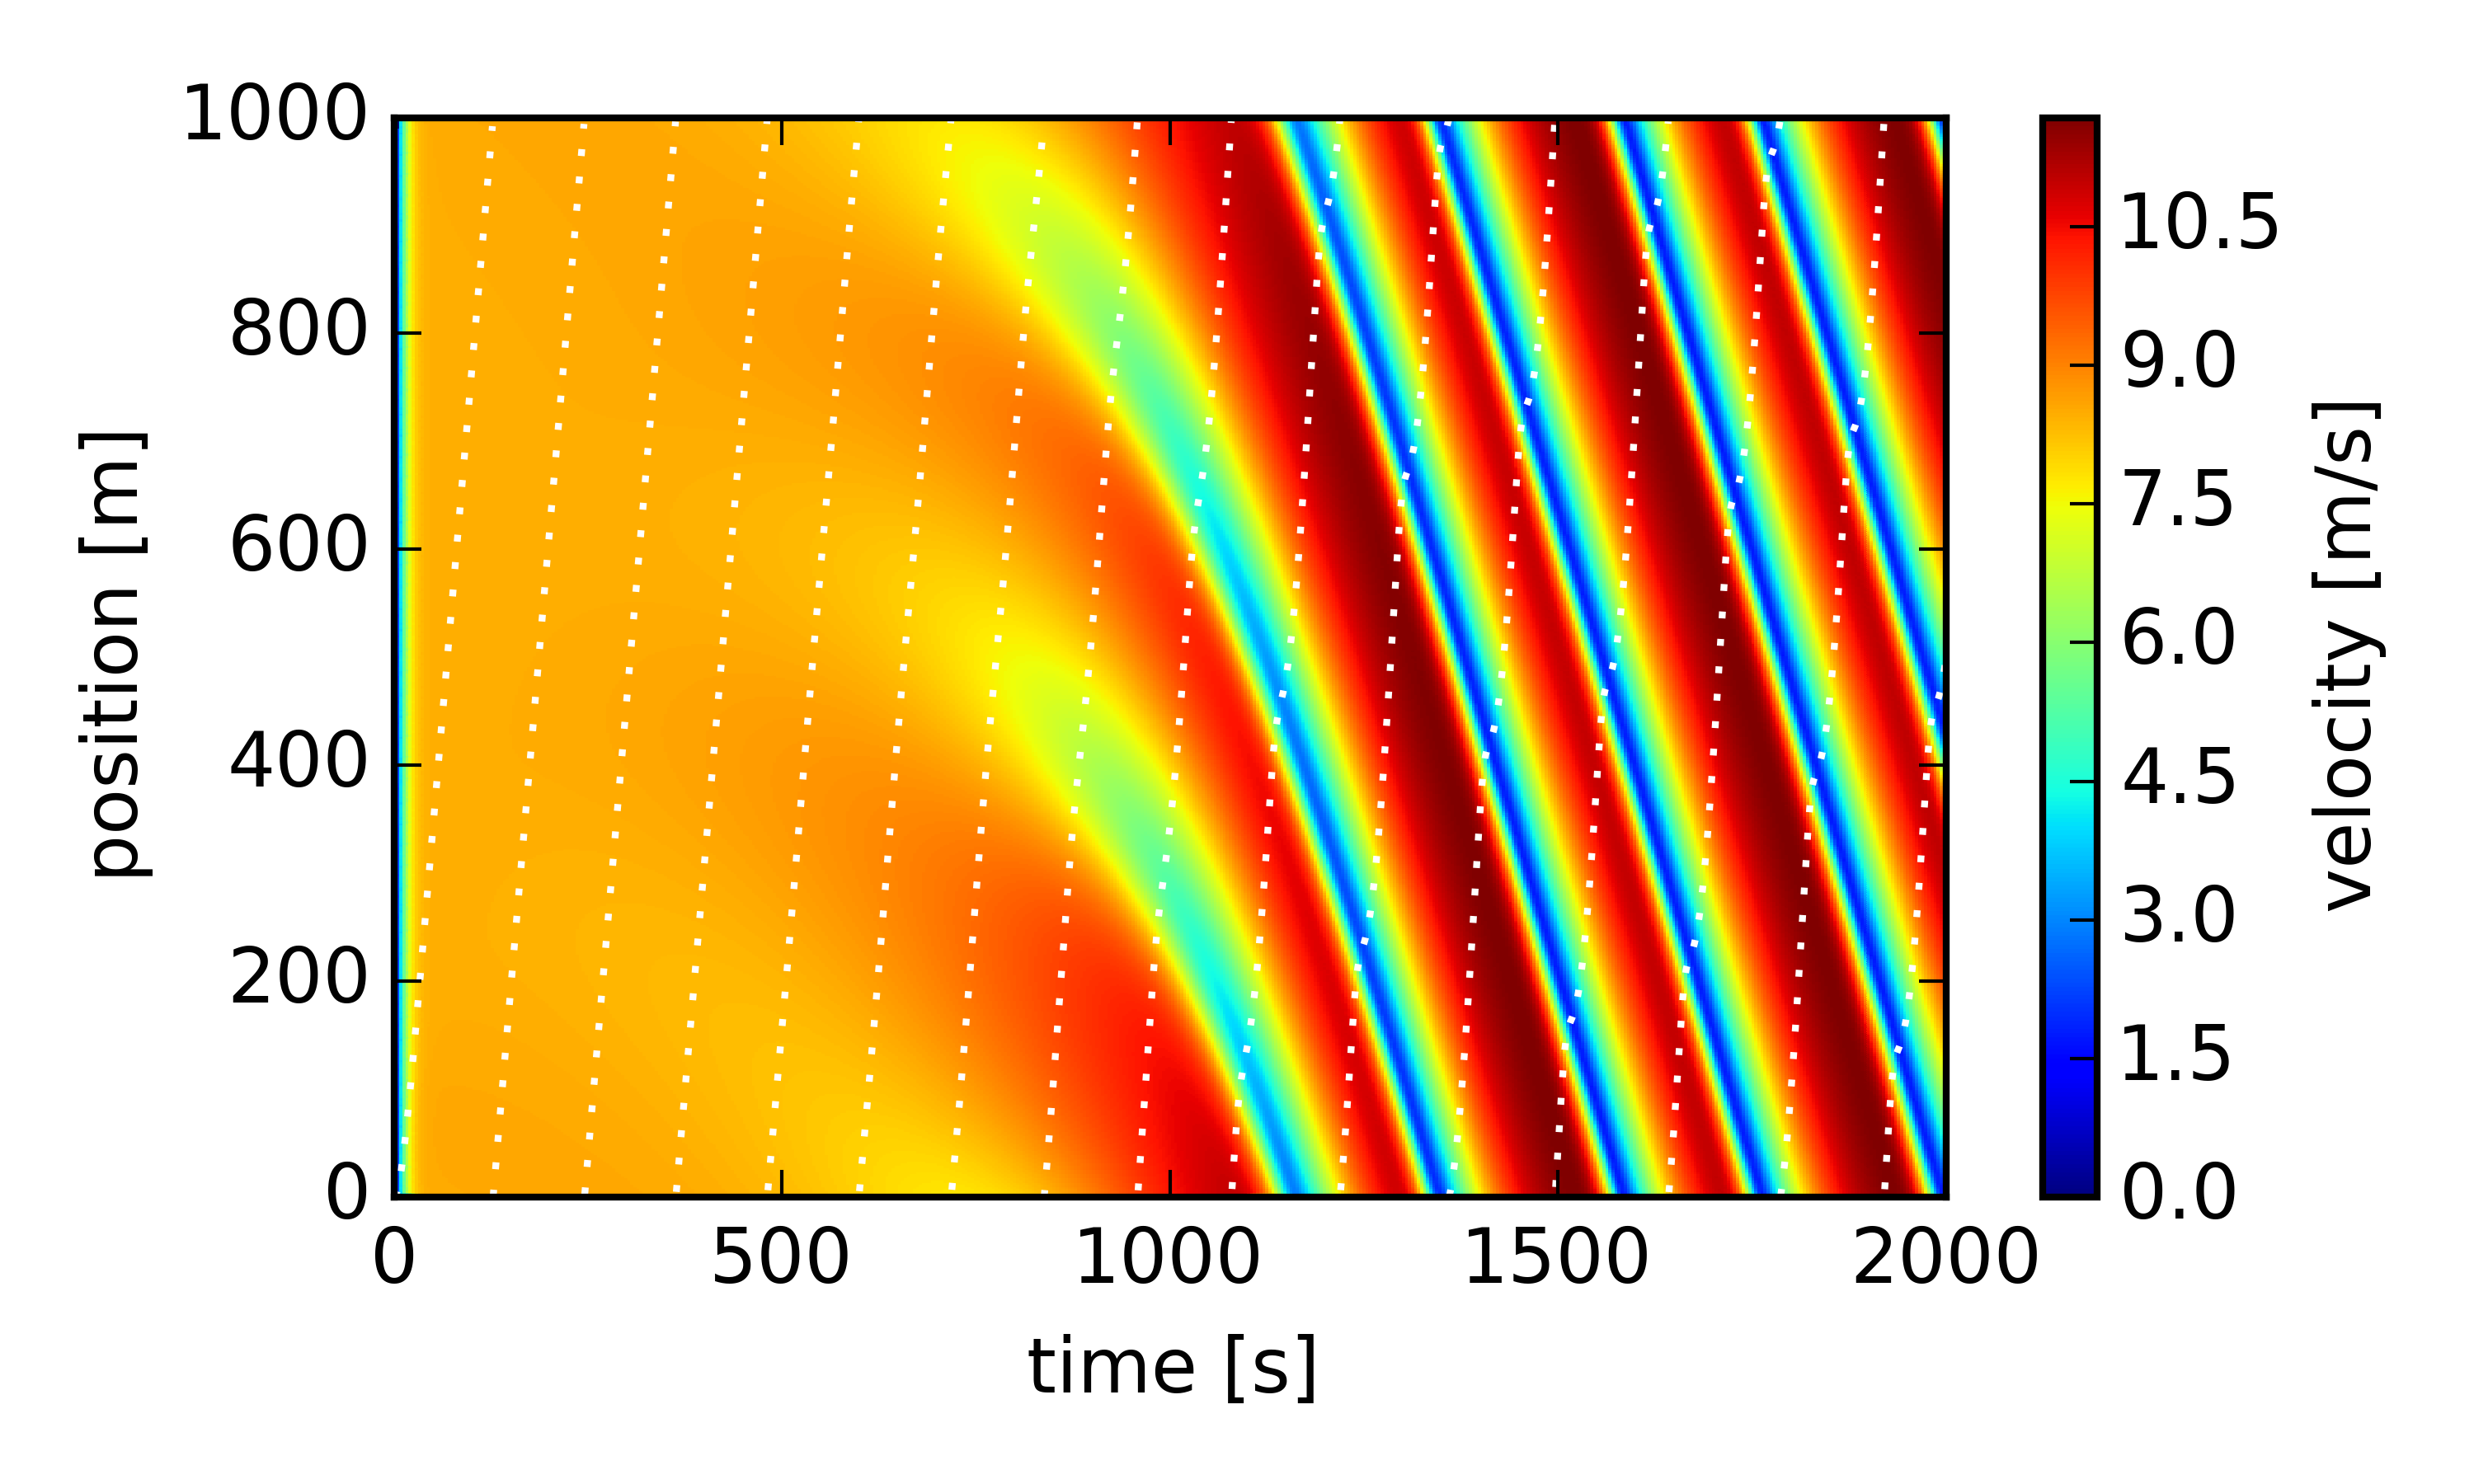
\includegraphics[width=5in]{../img/free_road.png}
    \caption{Spatio-temporal plot of the velocity field with stop-and-go waves. The dotted lines trace the trajectory of a selected car. The $N=50$ vehicles start uniformly distributed along the road. They quickly reach the equilibrium velocity (\SI{\sim 9}{m/s}). After about $t\approx\SI{700}{s}$ the instabilities start to become noticeable, and continue growing until $t\approx \SI{1100}{s}$. Note that the road is assumed to be periodic, hence the stop-and-go-waves, which leave the plot at the bottom, reappear at the top. Also note that the waves travel upstream, i.e. against the flow. For this simulation a time step $\Delta t=\SI{0.125}{s}$ was used.}
    \label{fig:free_road}
\end{figure}


\subsection{Effects of the interaction exponent $\gamma$}
We find that by increasing the exponent $\gamma$, the instabilities vanish. All the vehicles' velocity and spacing remain equalized to their equilibrium value. The transition from flow prone to instability and homogeneous traffic as a function of $\gamma$ is very sharp. Figure \ref{fig:order_param} shows this relation. To obtain this plot, for each value of $\gamma$, the simulation was run for a long time ($t_\mathrm{end} = \SI{500}{min}$), and then standard deviation of the final velocity distribution was computed as measure for inhomogeneity. As the standard deviation of the velocities vanishes in the homogeneous (disordered) phase, and quickly rises in the inhomogeneous (ordered) phase, it qualifies as an order parameter.

The critical value $\gamma_c$ at which the transition occurs is well defined and seems at most weakly dependent on the length of the road.
\begin{figure}
    \centering
    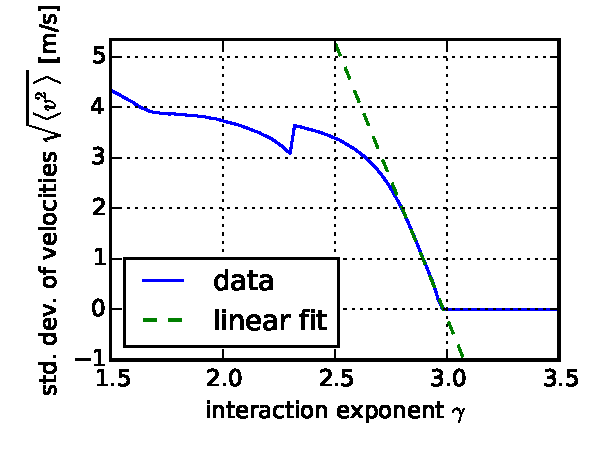
\includegraphics[width=4in]{../img/order_parameter.pdf}
    \caption{Plot of the standard deviation of the velocities of the vehicles at the end of the simulation as a function of the exponent $\gamma$. If the traffic remains stable, the velocities are equalized, and hence the variance vanishes. Increasing $\gamma$ beyond a critical value (here $\gamma_c \approx 0.298$) suppresses any instability. The transition appears as a sharp kink in the curve. For this plot, the vehicle density was fixed to $N/L=\SI{50}{km^{-1}}$.}
    \label{fig:order_param}
\end{figure}

Having established that tuning $\gamma$ gives rise to a sharp transition between phases, it stands to reason to map out this phase boundary as a function of another important parameter. Of particular interest is the density of vehicles, which has also been shown to be responsible for such a phase transition. The result can be seen in figure \ref{fig:phase_diagram}. For this the vehicle density was swept, while the corresponding critical exponent $\gamma_c$ was then determined via binary search.
\begin{figure}
    \centering
    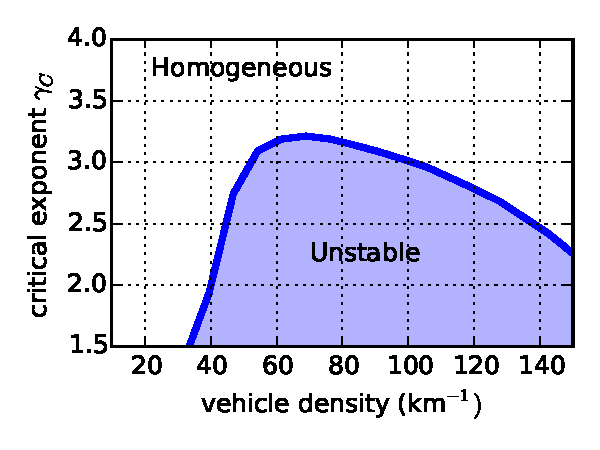
\includegraphics[width=4in]{../img/phase_diagram.pdf}
    \caption{Stability phase diagram with the mean vehicle density on the horizontal axis, and the interaction exponent on the vertical axis. While for the traditional value of $\gamma=2$ the traffic is unstable for a broad range of densities, a higher value of $\gamma$ can render the flow stable at high densities. For the chosen acceleration and deceleration parameters (here $a=\SI{0.6}{m/s^2}$ and $b=\SI{1.5}{m/s^2}$) the flow can be made stable unconditional on the vehicle density.}
    \label{fig:phase_diagram}
\end{figure}
\clearpage